
%\section{Using an SD Card Reader}
%	
%	Some of us succeeded in incorporating a SD card into our Arduino based instruments. But today we will revisit this. To do this we will need a SD card and to wire up an SD card breakout board.
%	\begin{figure}[h!] 
%	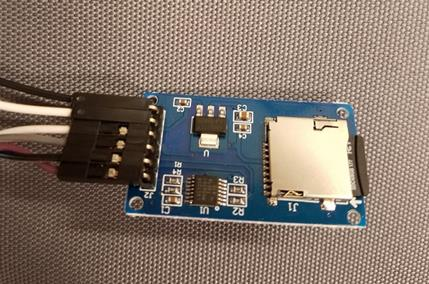
\includegraphics[width=3.614in,height=2.3981in]{PH4CAX47}
%	\end{figure}
%	Recall that there are six pins on our SD card reader board. Those six pins need to be wired to the following Arduino pins:
%	
%	\begin{equation*}
%	\begin{tabular}{ll}
%	SD Card Reader & Arduino \\ 
%	GND & GND \\ 
%	VCC & +5V \\ 
%	MISO & Pin 12 \\ 
%	MOSI & Pin 11 \\ 
%	SCK & Pin 13 \\ 
%	CS & Pin 4%
%	\end{tabular}%
%	\end{equation*}
%	
%	The pin names on the SD card reader board are usually on the back of the card.\begin{figure}[h!]
%		
%	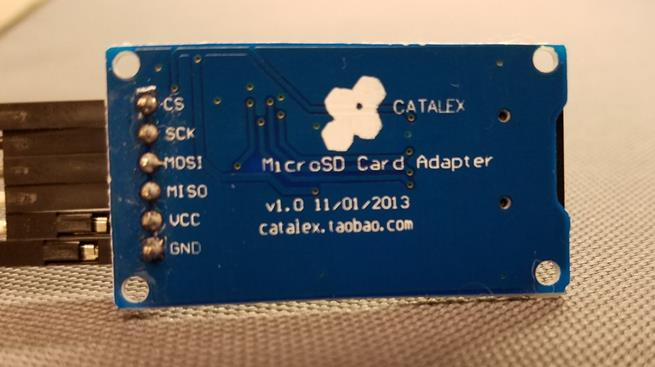
\includegraphics[width=4.5152in,height=2.5365in]{PH4CAX48}
%	\end{figure} \begin{figure}[h!]
%	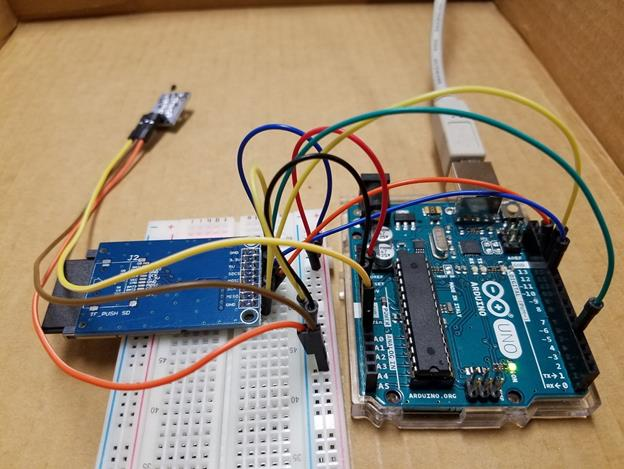
\includegraphics[width=4.1917in,height=3.1548in%
%	]{PH4CAX49}
%	\end{figure}
%	This figure includes a sensor, in this case a temperature sensing thermistor. Of course, we will need a sketch to tell the Arduino what to do with this new hardware. Here is an example:
%	
%	\bigskip
%	\begin{verbatim}
%	//////////////////////////////////////////////////////////////////////////////////////////
%	//////////////////////////////////////////////////////////////////////////////////////////
%	// DataLogger that gives time and voltage and saves it to a SD card.
%	//   
%	//////////////////////////////////////////////////////////////////////////////////////////
%	// Two input simple voltmeter 
%	// will measure 0 to 5V only!
%	// Voltages outside 0 to 5V will destroy your Arduino!!!
%	//////////////////////////////////////////////////////////////////////////////////////////
%	////Load Libraries//////////////////////////////////////////////////////////
%	  #include <SPI.h>     // Serial Peripheral Interface
%	  #include <SD.h>      // SD card library
%	//DEFINE VARIABLES///////////////////////////////////////////////////////////////////////
%	  const int CS_Pin = 4;       // this sets the pin for the CS connection
%	                             // to the SD card reader
%	// we want to have voltage vs time, so make a place to store a time value
%	   unsigned long time;
%	   int delayTime = 1000;    // time to wait in between data points.
%	 // make some integer variables that identify the analog input pins we will use:
%	   int AI0 = 0;
%	   int AI1 = 1;
%	// you also need a place to put the analog to digital converter values 
%	// from the Arduino
%	   int ADC0 = 0;
%	   int ADC1 = 0;
%	// Remember we will have to convert from Analog to digital converter(ADC) units
%	// to volts. We need our delta_V_min just like we did in lab 3 
%	   float delta_v_min=0.0049;   // volts per A2D unit
%	// We need a place to put the calculated voltage
%	   float voltage = 0.0;
%	 
%	 //SETUP/////////////////////////////////////////////////////////////////////////
%	   void setup() {
%	      // Open serial communications and wait for port to open:
%	      Serial.begin(9600);    // the 9600 tells our Arduino how fast to send data
%	      // Check to see if the serial port is working      
%	      while (!Serial) {
%	          ; // wait for serial port to connect. 
%	            // If it is, just keep going (don't do anything)
%	      }
%	      // Send a message to the Serial Monitor telling us that we are starting
%	      //     to use the SD card.
%	      Serial.print("Initializing SD card...");
%	      // See if the card is present and can be initialized.
%	      //    If there is a problem, tell us using the serial monitor.
%	     if (!SD.begin(CS_Pin)) {
%	         Serial.println("Card failed, or not present");
%	         // it didn't start the SD card write, so don't do anything more:
%	         return;
%	     }
%	     // But if the SD card did initialize, tell us on the serial monitor.
%	     Serial.println("card initialized.");
%	   }
%	 
%	//LOOP/////////////////////////////////////////////////////////////////////////
%	   void loop() {
%	   // We will have to turn our voltage numbers into text to send to our file
%	   // let's make a text variable (called a string) for this
%	      String dataString = ""; 
%	   // Read in the voltages in A2D units form the serial port
%	      ADC0 = analogRead(AI0); 
%	      ADC1 = analogRead(AI1);
%	 
%	   // Convert the voltage across the test resistor to voltage 
%	   //   units using delta_v_min
%	      voltage = (ADC1-ADC0) * delta_v_min;
%	 
%	   // get the time stamp
%	      time = millis();
%	 
%	   // make an output string that has the time and voltage
%	      dataString = dataString + String(time) + ", " + String(voltage);
%	     
%	   // open the file. note that only one file can be open at a time,
%	   // so you have to close this one before opening another.
%	      File dataFile = SD.open("datalog.txt", FILE_WRITE);
%	   // If the file is available, write to it, but then close it 
%	   //   right after. We will only keep the file open while we are 
%	   //   writing to it. This is safer. It helps prevent getting files 
%	   //   corrupted, and let's the Arduino keep adding to the file after 
%	   //   a problem.
%	      if (dataFile) {
%	        // print our data point
%	        dataFile.println(dataString);
%	         // close the file for safety
%	        dataFile.close();
%	         // print to the serial monitor too:
%	        Serial.println(dataString);
%	     }
%	     // if the file isn't open, pop up an error:
%	    else {
%	        Serial.println("error opening datalog.txt");
%	    }
%	    delay(delayTime);
%	   }
%	//////////////////////////////////////////////////////////////////////////////////////////
%	//////////////////////////////////////////////////////////////////////////////////////////   
%	 
%	 
%	\end{verbatim}
%	
%	Make sure you understand each line of this code does. We will modify this to include a special sensor today. So you will need to understand exactly what it does. It is a little fancy in that it tries to check to make sure the file is working properly and warns you if something is wrong. But most of the code is comments. So don't be discouraged by the length.
%	
%	Note that this is a very basic sketch. You should consider improving this sketch (there will be suggestions in the lab assignment below). You may need to improve this sketch for your group project.
%
%\section{Time Stamping}
%
%	Very often, we need to know exactly when a data point was taken. We saw this in our RC circuit lab. Saving data to a SD card could be more useful if we knew the collection time of each data point and could save that along with the data point, itself. We could use a stop watch and write it down, but that defeats our goal of having the computer do the data collection. We want the Arduino system to be able to do this on it's own. To do that, we need to add another hardware piece to our data logger. We need to add a clock. 
%	
%	There is a breakout board that is a stand-alone clock. It has it's own battery that keeps the clock going when the rest of the instrument is turned off. When the Arduino starts up, the data logger code can get the time from the breakout board clock. This will allow the data logger to know the exact time for each measurement and to place a time stamp on that measurement when the data point is recorded. These breakout boards are called Real Time Clocks (RTC) and the ones we have are the Adafruit DS3231 Precision RTC breakout boards (https://www.adafruit.com/product/3013).
%	\begin{figure}[h!]
%	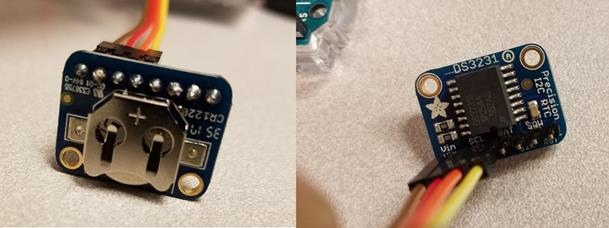
\includegraphics[width=5.1214in,height=1.9294in]{PH4CAX4A}
%	\end{figure}
%
%\section{Connecting the RTC to an Arduino}
%	
%	The real time clock uses the I2c bus on the Arduino. A \textquotedblleft bus\textquotedblright\ is a set of pins that can be used by more than one instrument at a time. Each instrument has a special code or \textquotedblleft address\textquotedblright\ to identify it. In your Arduino code, you use this address to tell the Arduino processor which instrument to get data from.
%	
%	The RTC only needs four wires. The wiring is as follows:
%	
%	\begin{equation*}
%	\begin{tabular}{ll}
%	RTC & Arduino \\ 
%	Vcc & 3.3V \\ 
%	GND & GND \\ 
%	SCL & SCL \\ 
%	SDA & SDA%
%	\end{tabular}%
%	\end{equation*}
%	
%	Since this is an Adafruit product, there is a nice tutorial on wiring up the RTC and a library to download and use to make it run (https://learn.adafruit.com/adafruit-ds3231-precision-rtc-breakout/). The Adafruit example code is shown below. I have commented out the section that would set the clock. Hopefully your clock will already be set, so you won't use that part of the code. If not, ask for help from your Instructor or TA.
%	
%	\bigskip
%	\begin{verbatim}
%	// Date and time functions using a DS3231 RTC connected via I2C and Wire lib
%	#include <Wire.h>
%	#include "RTClib.h"
%	 
%	RTC_DS3231 rtc;
%	 
%	char daysOfTheWeek[7][12] = {"Sunday", "Monday", "Tuesday", 
%	    "Wednesday", "Thursday", "Friday", "Saturday"};
%	 
%	void setup () {
%	  Serial.begin(9600); // set up the serial port
%	  delay(3000); // wait for console opening
%	  // now let's start communication with the real time clock
%	  if (! rtc.begin()) {
%	    Serial.println("Couldn't find RTC");
%	    while (1);
%	  }
%	 
%	/* We will use a Raspberry Pi to set all the clocks ahead of time so we won't
%	   Do this part
%	  if (rtc.lostPower()) {
%	    Serial.println("RTC lost power, lets set the time!");
%	    // following line sets the RTC to the date & time this sketch was compiled
%	    rtc.adjust(DateTime(F(__DATE__), F(__TIME__)));
%	    // This line sets the RTC with an explicit date & time, for example to set
%	    // January 21, 2014 at 3am you would call:
%	    // rtc.adjust(DateTime(2014, 1, 21, 3, 0, 0));
%	    }
%	 */ 
%	  
%	}
%	 
%	void loop () {
%	    // use the RTC to get the time
%	    DateTime now = rtc.now();
%	    
%	    // now print out the time in various ways.
%	    Serial.print(now.year(), DEC);
%	    Serial.print('/');
%	    Serial.print(now.month(), DEC);
%	    Serial.print('/');
%	    Serial.print(now.day(), DEC);
%	    Serial.print(" (");
%	    Serial.print(daysOfTheWeek[now.dayOfTheWeek()]);
%	    Serial.print(") ");
%	    Serial.print(now.hour(), DEC);
%	    Serial.print(':');
%	    Serial.print(now.minute(), DEC);
%	    Serial.print(':');
%	    Serial.print(now.second(), DEC);
%	    Serial.println();
%	    
%	    Serial.print(" since midnight 1/1/1970 = ");
%	    Serial.print(now.unixtime());
%	    Serial.print("s = ");
%	    Serial.print(now.unixtime() / 86400L);
%	    Serial.println("d");
%	    
%	    // We also don't need the next part, but it is interesting to know
%	    //  that you can do time calculations with the RTC library functions.
%	    // calculate a date which is 7 days and 30 seconds into the future
%	    DateTime future (now + TimeSpan(7,12,30,6));
%	    
%	    Serial.print(" now + 7d + 30s: ");
%	    Serial.print(future.year(), DEC);
%	    Serial.print('/');
%	    Serial.print(future.month(), DEC);
%	    Serial.print('/');
%	    Serial.print(future.day(), DEC);
%	    Serial.print(' ');
%	    Serial.print(future.hour(), DEC);
%	    Serial.print(':');
%	    Serial.print(future.minute(), DEC);
%	    Serial.print(':');
%	    Serial.print(future.second(), DEC);
%	    Serial.println();
%	    
%	    Serial.println();
%	    delay(3000);
%	}
%	\end{verbatim}
%	
%	\bigskip
%	
%	You will need to modify today's data logger code to use the RTC. You can do this by reading the example code and figuring out how it prints the time. Then modify this to print to our SD card instead of the serial port. 
%	
%	For our final group designed lab, you will likely want a RTC. Because our real time clocks will have to eventually be resent, it is probably not a good idea to solder the breakout board directly into your instrument.